\section{Лекция 20.02.2020}

\begin{comment}
    Для $F = \CC$ всякую квадратичную форму можно привести к виду \eqref{lec21:1}, где $k = \rk Q$.
    \begin{equation}
        \label{lec21:1}
        Q = x_1^2 + \dots + x_k^2
    .\end{equation}
\end{comment}


\subsection{Положительный и отрицательный индексы инерции квадратичной формы над $\RR$}

Пусть $F = \RR$.

Пусть $Q \colon V \to \RR$ --- квадратичная форма.

Можно привести к нормальному виду
\begin{equation*}
    Q(x_1, \dots, x_n) = x_1^2 + \dots + x_s^2 - x_{s + 1}^2 - \dots - x_{s + t}^2
.\end{equation*}

Здесь
\begin{math}
    \begin{aligned}[t]
        &i_+ := s \text{ --- положительный индекс инерции квадратичной формы $Q$}, \\
        &i_- := t \text{ --- отрицательный индекс инерции квадратичной формы $Q$}.
    \end{aligned}
\end{math}


\subsection{Закон инерции}

\begin{theorem}
    Числа $i_+$ и $i_-$ не зависят от базиса в котором $Q$ принимает нормальный вид.
\end{theorem}

\begin{proof}
    $s + t = \rk Q$, то есть не зависит от выбора базиса. Следовательно, достаточно показать, что число $s$ определено однозначно.

    Пусть $\E = (e_1, \dots, e_n)$ --- базис, в котором $Q$ принимает нормальный вид
    \begin{equation*}
        Q = x_1^2 + \dots + x_s ^2 - x_{s + 1}^2 - \dots - x_{s + t}^2
    .\end{equation*}

    Пусть $\E' = (e'_1, \dots, e'_n)$ --- другой базис, в котором $Q$ принимает нормальный вид
    \begin{equation*}
        Q = x'^2_1 + \dots + x'^2_{s'} - x'^2_{s' + 1} - \dots - x'^2_{s' + t'}
    .\end{equation*}

    Предположим, что $s \neq s'$, можно считать что $s > s'$.

    Положим 
    \begin{math}
        \begin{aligned}[t]
            &L := \left< e_1, \dots, e_s \right>, \ \dim L = s, \\
            &L' := \left< e'_{s' + 1}, \dots, e'_n \right>, \ \dim L' = n - s'.
        \end{aligned}
    \end{math}

    \bigskip
    Так как $L + L' \subseteq V$, то $\dim \left(L + L'\right) \leq n$.

    Тогда, $\dim \left(L \cap L'\right) \geq s + (n - s') - n = s - s' > 0$.

    \bigskip
    Значит, $\exists$ вектор $v \in L \cap L'$, такой что $v \neq 0$.

    Теперь: 
    \begin{enumerate}[nosep]
        \item Так как $v \in L$, то $Q(v) > 0$,
        \item Так как $v \in L'$, то $Q(v) \leq 0$.
    \end{enumerate}
 
    Противоречие.
\end{proof}


\subsection{Следствие метода Якоби о вычислении индексов инерции квадратичной формы над $\RR$}

Пусть $Q \colon V \to \RR$ --- квадратичная форма,

$\E = (e_1, \dots, e_n)$ --- базис,

$B = B(Q, \E)$, 

$\delta_k$ --- $k$-й угловой минор матрицы $B$.


\begin{corollary}[из метода Якоби]
    Пусть $\delta_k \neq 0 \ \forall k$. Тогда:

    Число $i_+$ равно количеству \underline{сохранений знака} в последовательности $1, \delta_1, \dots, \delta_n$.

    Число $i_-$ равно количеству \underline{перемен знака} в последовательности $1, \delta_1, \dots, \delta_n$.
\end{corollary}

\begin{proof}
    Метод Якоби $ \implies \exists $ базис, в котором $Q$ принимает канонический вид
    \begin{equation*}
        Q = \delta_1 x_1^2 + \frac{\delta_2}{\delta_1} x_2^2 + \dots + \frac{\delta_n}{\delta_{n - 1}} x_{n}^2
    .\end{equation*}

    Здесь, знак отношения $\frac{\delta_i}{\delta_{i - 1}}$ соответствует смене либо сохранению знака в рассматриваемой последовательности.

    По закону инерции, количества знаков $+$ и $-$ не изменяются от выбора базиса.
\end{proof}


\subsection{Положительно определённые, отрицательно определённые, неотрицательно определённые, неположительно определённые, неопределённые квадратичные формы над $\RR$}

\begin{definition}
    Квадратичная форма $Q$ над $\RR$ называется
\end{definition}
\begin{table}[H]
{\renewcommand{\arraystretch}{1.7}
    \begin{tabular}{c|c|c|c|c}
        Термин & Обозначение & Условие & Нормальный вид & Индексы инерции \\ \hline
        Положительно определённой & $Q > 0$ & $Q(x) > 0 \ \forall x \neq 0$ & $x_1^2 + \dots + x_n^2$ & $i_+ = n, i_- = 0$ \\ \hline
        Отрицательно определённой & $Q < 0$ & $Q(x) < 0 \ \forall x \neq 0$ & $-x_1^2 - \dots - x_n^2$ & $i_+ = 0, i_- = n$ \\ \hline
        Неотрицательно определённой & $Q \geq 0$ & $Q(x) \geq 0 \ \forall x$ & $x_1^2 + \dots + x_k^2, \ k \leq n$ & $i_+ = k, i_- = 0$ \\ \hline
        Неположительно определённой & $Q \leq 0$ & $Q(x) \leq 0 \ \forall x$ & $-x_1^2 - \dots - x_k^2, \ k \leq n$ & $i_+ = 0, i_- = k$ \\ \hline
        Неопределённой & --- & 
        \begin{math}
            \begin{aligned}
                \exists x : Q(x) > 0 \\
                \exists y : Q(y) < 0
            \end{aligned}
        \end{math} &
        \begin{math}
            \begin{gathered}
                x_1^2 + \dots + x_s ^2 - x_{s + 1}^2 - x_{s + t}^2 \\
                s, t \geq 1
            \end{gathered}
        \end{math} & $i_+ = s, i_- = t$
        \\ \hline
    \end{tabular}       
}
\end{table}


\subsection{Примеры}

$V = \RR^2$.

\begin{enumerate}
\item $Q(x, y) = x^2 + y^2$, $Q > 0$.

    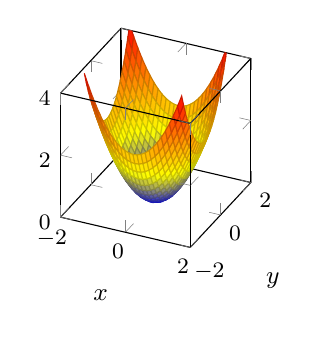
\begin{tikzpicture}
    \begin{axis}[
    xlabel=$x$, ylabel=$y$, small,
    xmin=-2, xmax=2,
    ymin=-2, ymax=2,
    zmin=0, zmax=4,
    3d box=complete,
    unit vector ratio*=1 1 1,
    ]
    \addplot3[surf, domain=-1.5:1.5] 
    {x^2+y^2};
    \end{axis}
    \end{tikzpicture} 

\item $Q(x, y) = -x^2 - y^2$, $Q < 0$.

    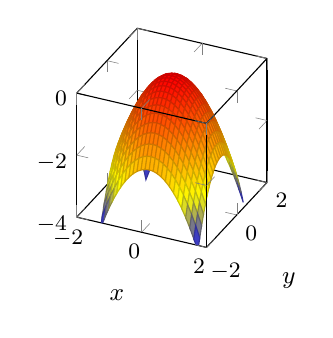
\begin{tikzpicture}
    \begin{axis}[
    xlabel=$x$, ylabel=$y$, small,
    xmin=-2, xmax=2,
    ymin=-2, ymax=2,
    zmin=-4, zmax=0,
    3d box=complete,
    unit vector ratio*=1 1 1,
    ]
    \addplot3[surf, domain=-1.5:1.5] 
    {-x^2-y^2};
    \end{axis}
    \end{tikzpicture} 

\item $Q(x, y) = x^2$, $Q \geq 0$.
    
    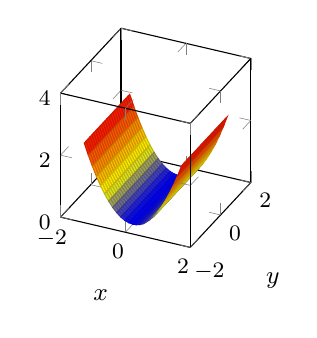
\begin{tikzpicture}
    \begin{axis}[
    xlabel=$x$, ylabel=$y$, small,
    xmin=-2, xmax=2,
    ymin=-2, ymax=2,
    zmin=0, zmax=4,
    3d box=complete,
    unit vector ratio*=1 1 1,
    ]
    \addplot3[surf, domain=-1.5:1.5] 
    {x^2};
    \end{axis}
    \end{tikzpicture} 

\item $Q(x, y) = -x^2$, $Q \leq 0$.

    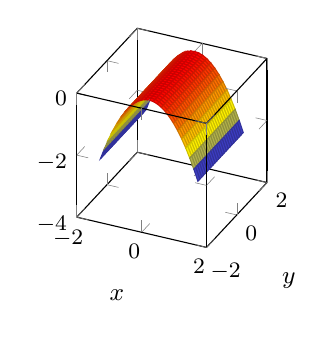
\begin{tikzpicture}
    \begin{axis}[
    xlabel=$x$, ylabel=$y$, small,
    xmin=-2, xmax=2,
    ymin=-2, ymax=2,
    zmin=-4, zmax=0,
    3d box=complete,
    unit vector ratio*=1 1 1,
    ]
    \addplot3[surf, domain=-1.5:1.5] 
    {-x^2};
    \end{axis}
    \end{tikzpicture} 

\item $Q(x, y) = x^2 - y^2$.

    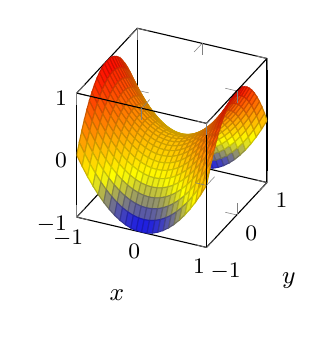
\begin{tikzpicture}
    \begin{axis}[
    xlabel=$x$, ylabel=$y$, small,
    xmin=-1, xmax=1,
    ymin=-1, ymax=1,
    zmin=-1, zmax=1,
    3d box=complete,
    unit vector ratio*=1 1 1,
    ]
    \addplot3[surf, domain=-1:1] 
    {x^2 - y^2};
    \end{axis}
    \end{tikzpicture} 

\end{enumerate}


\subsection{Одно применение квадратичных форм над $\RR$}

\href{https://www.dropbox.com/s/wwv38znnuts9rld/Qforms_application.pdf?dl=0}{Презентация} (продублирована ниже)

\subsubsection{Знаем из курса математического анализа}

Пусть $f\colon \RR \to \RR$ --- некоторая функция, $x_0 \in \RR$ --- некоторая точка.

Если $f$ дважды дифференцируема в точке $x_0$, то для малого приращения $y$ имеем
\begin{equation*}
    f(x_0 + y) = f(x_0) + ay + by^2 + o(y^2)
,\end{equation*}
где $a = f'(x_0)$, $b = f''(x_0) / 2$.

\begin{proposal}[необходимое условие локального экстремума]
    Если $f$ в точке $x_0$ имеет локальные экстремум, то $f'(x_0) = 0$.
\end{proposal}

\begin{proposal}[достаточные условия локального экстремума]
    Пусть $f'(x_0) = 0$. Тогда
    \begin{itemize}[nosep]
    \item если $f''(x_0) > 0$, то $f$ в точке $x_0$ имеет локальный минимум;
    \item если $f''(x_0) < 0$, то $f$ в точке $x_0$ имеет локальный максимум.
    \end{itemize}
\end{proposal}

\subsubsection{Применение квадратичных форм}

Пусть $f\colon \RR^n \to \RR$ --- некоторая функция, $x_0 \in \RR^n$ --- некоторая точка.

Если $f$ <<дважды дифференциируема>> в точке $x_0$, то для малого приращения $y = \begin{pmatrix} y_1 \\ \dots \\ y_n \end{pmatrix} \in \RR^n$ имеем

\begin{equation*}
    f(x_0 + y) = f(x_0) + \underbrace{a_1 y_1 + \dots + a_n y_n}_{l(y)} + \underbrace{\sum_{i = 1}^{n} b_{ii} y_i^2 + \sum_{1 \leq i < j \leq n} 2b_{ij} y_i y_j}_{Q(y)} + o(|y|^2)
.\end{equation*}

$l(y)$ --- линейная форма, (называется <<дифференциал>>)

$Q(y)$ --- квадратичная форма.

\begin{proposal}[необходимое условие локального экстремума]
    Если $f$ в точке $x_0$ имеет локальный экстремум, то $l(y) \equiv 0$ (то есть $a_1 = \dots = a_n = 0$).
\end{proposal}

\begin{proposal}[достаточные условие локального экстремума или его отсутствия]
    Пусть $l(y) \equiv 0$. Тогда:
    \begin{itemize}[nosep]
    \item если $Q > 0$, то $f$ в точке $x_0$ имеет локальный минимум;
    \item если $Q < 0$, то $f$ в точке $x_0$ имеет локальный максимум;
    \item если $Q$ неопределённа, то $f$ в точке $x_0$ не имеет локального экстремума.
    \end{itemize}
\end{proposal}

\subsection{Критерий Сильвестра положительной определённости квадратичной формы}

Пусть 
\begin{math}
    \begin{aligned}[t]
        &V \text{ --- векторное пространство над $\RR$, $\dim V = n$}, \\
        &\E = (e_1, \dots, e_n) \text{ --- базис $V$}, \\
        &B = B(Q, \E), \\
        &B_k \text{ --- левый верхний $k \times k$ блок}, \\
        &\delta_k = \det B_k.
    \end{aligned}
\end{math}

\begin{theorem}[Критерий Сильвестра положительной определенности]
    \begin{equation*}
        Q > 0 \iff \delta_k > 0 \ \forall k = 1 \dots n
    .\end{equation*}
\end{theorem}

\begin{proof}~
    \begin{description}
    \item[$\impliedby$] По следствию из метода Якоби, $i_+ = n$, то есть $Q > 0$.
    \item[$\implies$] $Q > 0 \implies \exists C \in M_n^0(\RR)$, такая что $C^TBC = E$.

        Тогда, $\det C^T \cdot \underset{= \delta_n}{\det B} \cdot \det C = 1$. Отсюда, $\delta_n = \frac{1}{(\det C)^2} > 0$.

        Теперь, для любого $k$ ограничение $Q$ на $\left< e_1, \dots, e_k \right>$ тоже положительно определённо, а его матрица в базисе $e_1, \dots, e_k$ равна $B_k$. Следовательно, $\det B_k > 0$.
        \qedhere
    \end{description}
\end{proof}

\subsection{Критерий отрицательной определённости квадратичной формы}

\begin{corollary}
    \begin{equation*}
        Q < 0 \iff \delta_k \begin{cases}
            > 0 & \text{при } k \divby 2, \\
            < 0 & \text{при } k \!\!\not\;\divby 2.
        \end{cases}
    \end{equation*}
\end{corollary}

\begin{proof}
    \begin{math}
        \begin{aligned}[t]
            Q < 0 &\iff -Q > 0 \\
                  &\iff \det (-B_k) > 0 \ \forall k \\
                  &\iff (-1)^{k} \delta_k > 0 \ \forall k
        \end{aligned}
    \end{math}
\end{proof}


\subsection{Евклидово пространство и скалярное произведение}

\begin{definition}
    \textit{Евклидово пространство} --- это векторное пространство $\EE$ над $\RR$, на котором задано \textit{скалярное произведение}, то есть такое отображение $(\bigcdot, \bigcdot)\colon \EE \times \EE \to \RR$, что
    \begin{enumerate}[nosep]
        \item $(\bigcdot, \bigcdot)$ --- симметричная билинейная форма,
        \item Квадратичная форма $(x, x)$ положительно определённая.
    \end{enumerate}
\end{definition}


\subsection{Примеры}

\begin{enumerate}
\item 
    $\EE = \RR^n$, $x = \begin{pmatrix} x_1 \\ \dots \\ x_n \end{pmatrix}$, $y = \begin{pmatrix} y_1 \\ \dots \\ y_n \end{pmatrix}$.

    $(x, y) := x_1 y_1 + \dots + x_n y_n \leftarrow $ стандартное скалярное произведение в $\RR^n$.

    $(x, x) = x_1^2 + \dots + x_n^2 > 0$.

\item
    $\EE = \text{Mat}_{m \times n}(\RR)$,

    $(A, B) := \tr (A^{T} B)$,

    $(A, A) = \tr (A^{T}A) = \sum_{i = 1}^{m} \sum_{j = 1}^{m} a_{ij}^2$.

\item
    $\EE = C[a, b]$,
    
    $(f, g) := \int_a^b f(x) g(x) \mathop{}\!dx$,

    $(f, f) = \int_a^b f^2(x) \mathop{}\!dx > 0$.
\end{enumerate}
